\pagestyle{circuito}
\label{circuito}

\begin{textblock*}{5.625in}(0pt,0pt)%
\vspace*{-2.5cm}
\hspace*{-1.75cm}\includegraphics*[width=147mm]{./imgs/CIRCUITO.png}
\end{textblock*}

\pagebreak

\hspace{.5cm}

\begin{center}
\hspace{-.5cm}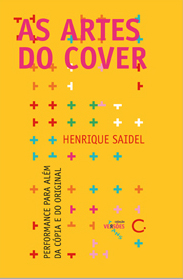
\includegraphics[width=45.4mm]{./imgs/cover.jpg}
\end{center}

\hspace*{-7cm}\hrulefill\hspace*{-7cm}

\medskip

\noindent{}Essa obra questiona a noção de origem, original, único, essência originária. Afinal, o que afirmamos quando dizemos que algo é original? Desde Aristóteles já sabemos que a imitação – ou mímesis – deveria recriar a potência de vida e não sua forma. É com base nesse pensamento que o autor pode afirmar que o cover cria {\slsc{COM}} sua base precedente e, sem qualquer hierarquia preestabelecida, inventa outro original.

%\hspace{.5cm}
\vfill

\hspace*{-.4cm}\begin{minipage}[c]{1\linewidth}
\small{
{\Formular{\textbf{
\hspace*{-.1cm}Título: As artes do cover\\
Autor: Henrique Saidel\\ 
Páginas: 352\\
Formato: 14x21cm\\
Preço: R\$ 55,00\\
ISBN: 978-85-9582-049-4\\
Disponibilidade: Disponível
}}}}
\end{minipage}

\pagebreak

\hspace{.5cm}

\begin{center}
\hspace*{-4cm}\raisebox{5.8cm}{\rotatebox[origin=t]{90}{\Formular{\textbf{Lançamento}}}}
\hspace*{4cm}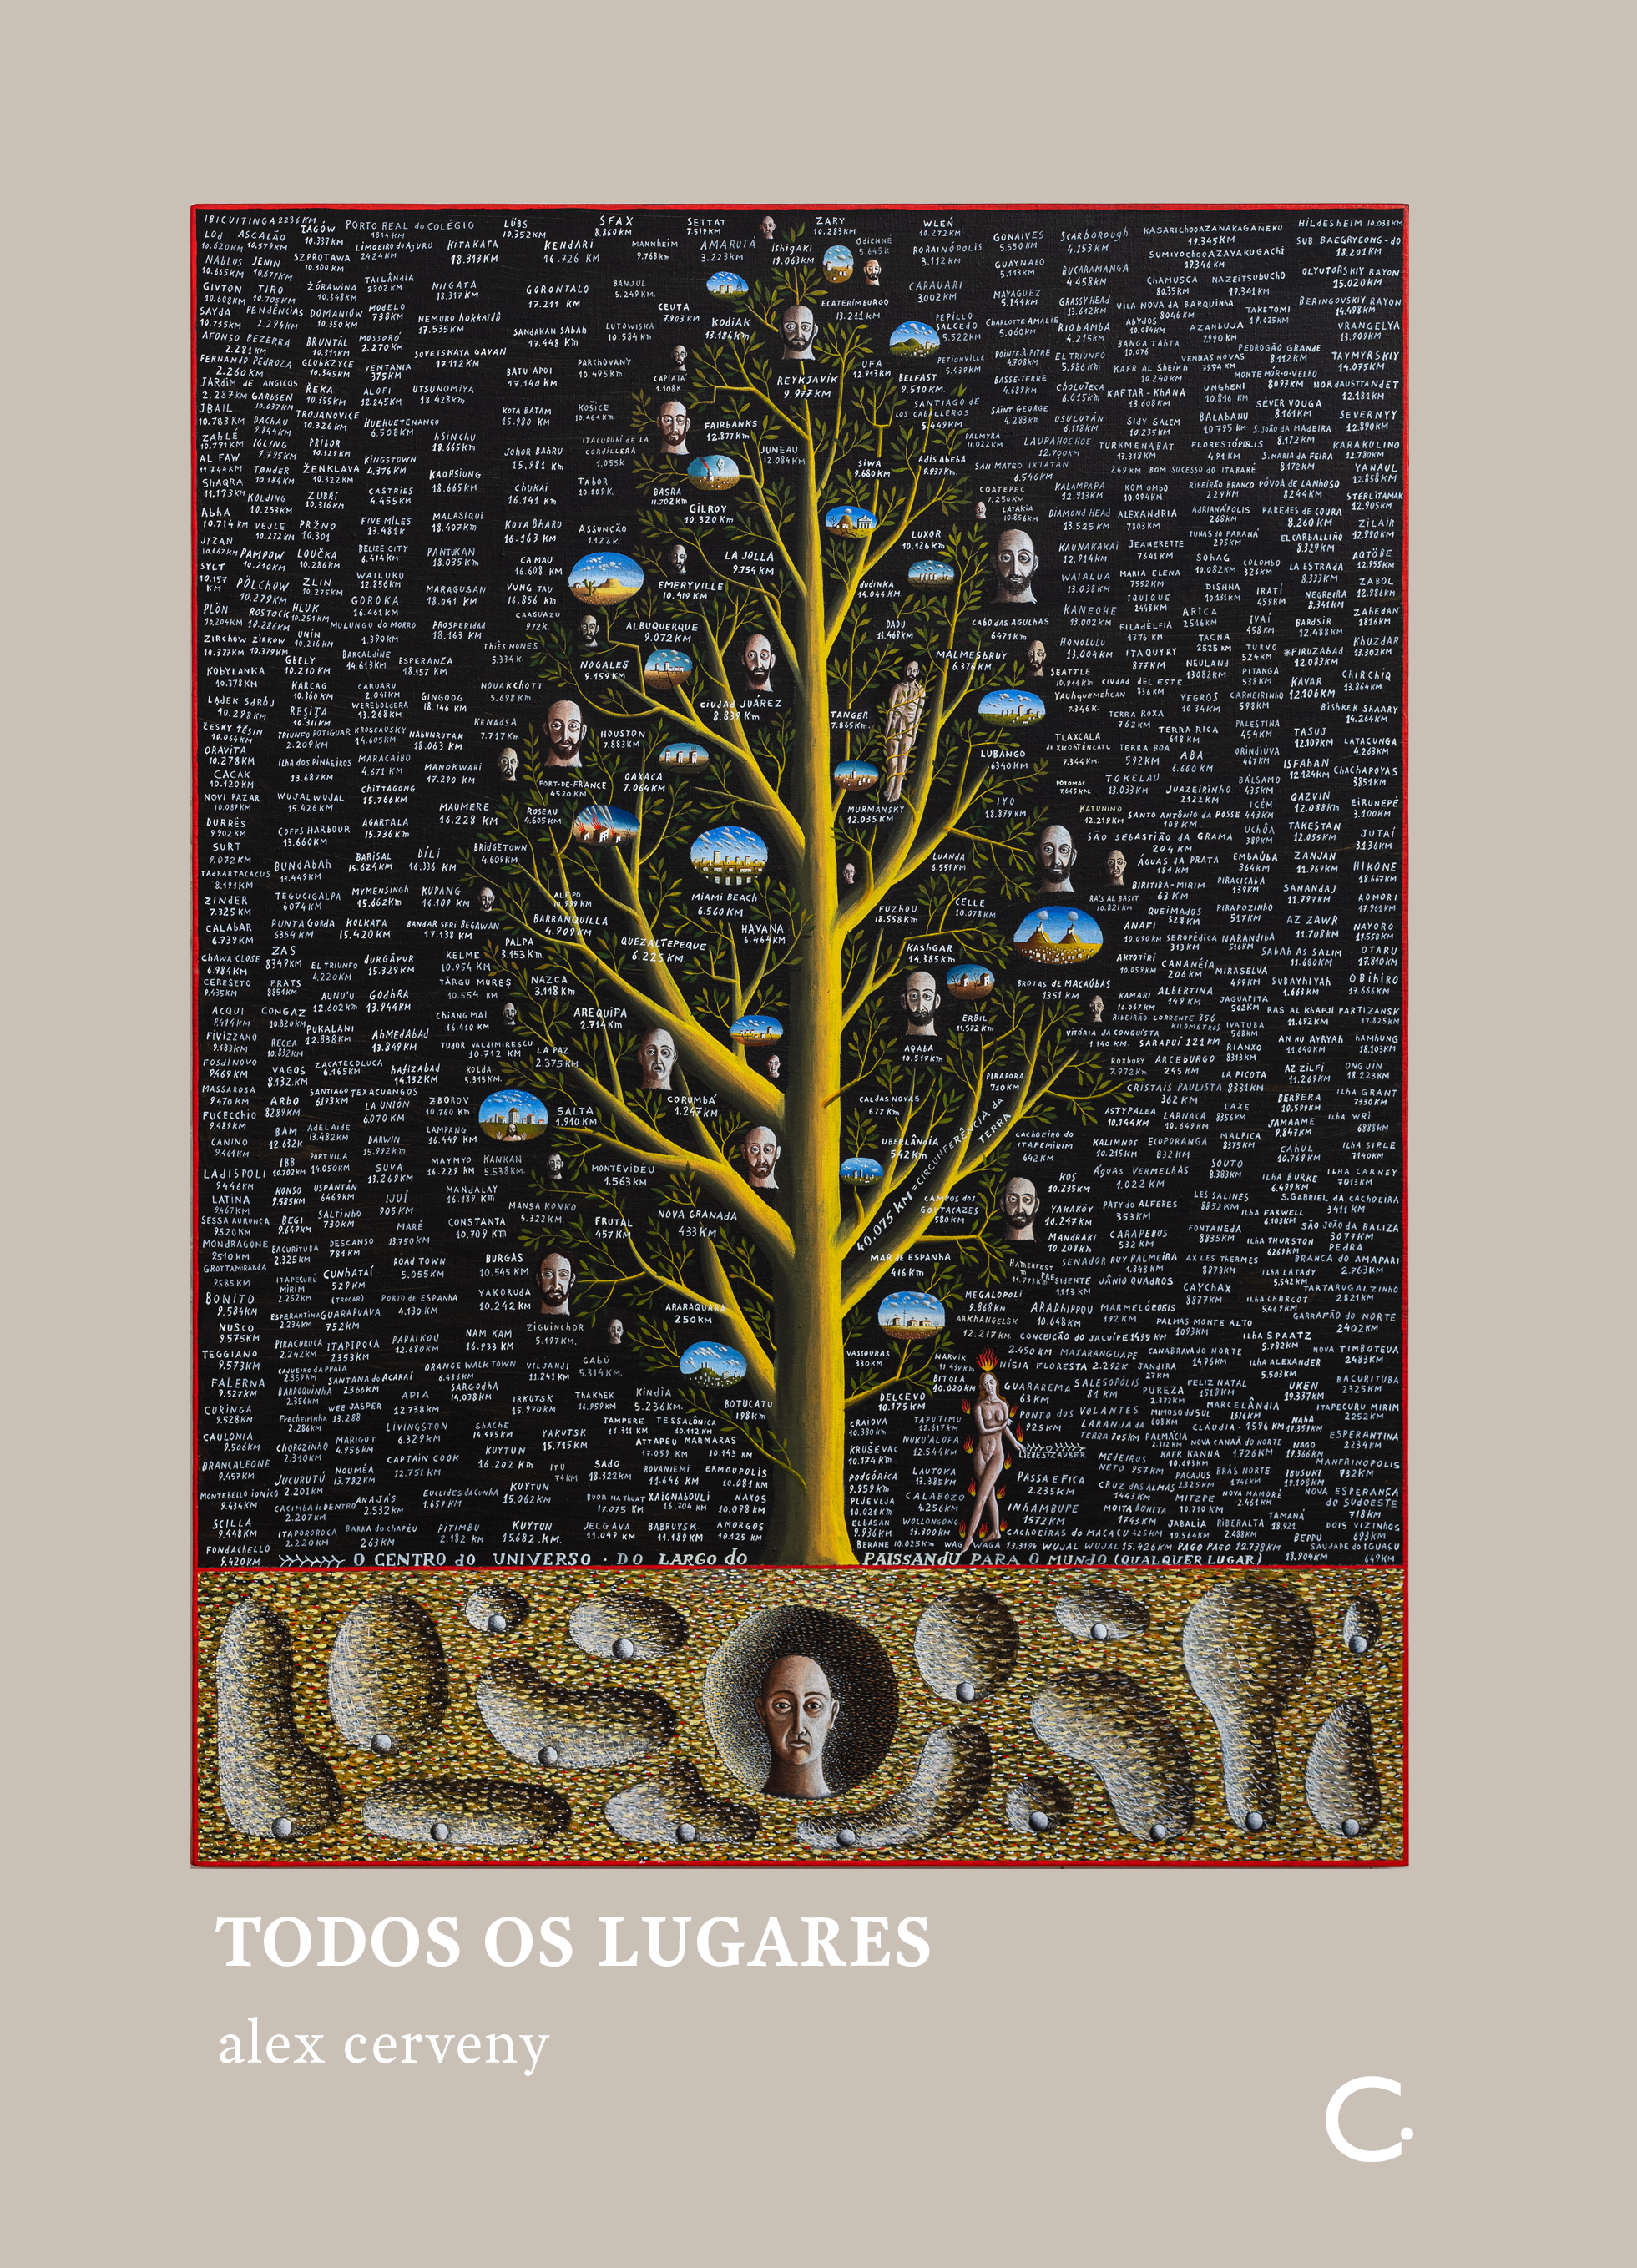
\includegraphics[width=50mm]{./imgs/lugares.jpg}
\end{center}

\hspace*{-7cm}\hrulefill\hspace*{-7cm}

\medskip

\noindent{}Um dos mais notáveis artistas brasileiros da atual geração, Ceverny produz em suas viagens peregrinações e inflexões sobre si próprio, dividindo na publicação uma vida rica, enlaçada cuidadosamente entre imagem e escrita, entre riscos, traços e viagens. O livro belo e singular conta com histórias e ilustrações do artista, além do prefácio do curador Renato Rezende, um posfácio do escritor e filósofo Rodrigo Petronio.


%\hspace{.5cm}
\vfill

\hspace*{-.4cm}\begin{minipage}[c]{1\linewidth}
\small{
{\Formular{\textbf{
\hspace*{-.1cm}Título: Todos os lugares\\
Autor: Alex Cerveny\\ 
Páginas: 190\\
Formato: 16x23cm\\
Preço: R\$ 80,00\\
ISBN: 978-85-9582-050-0\\
Disponibilidade: Em breve
}}}}
\end{minipage}

\pagebreak

\hspace{.5cm}

\begin{center}
\hspace*{-.5cm}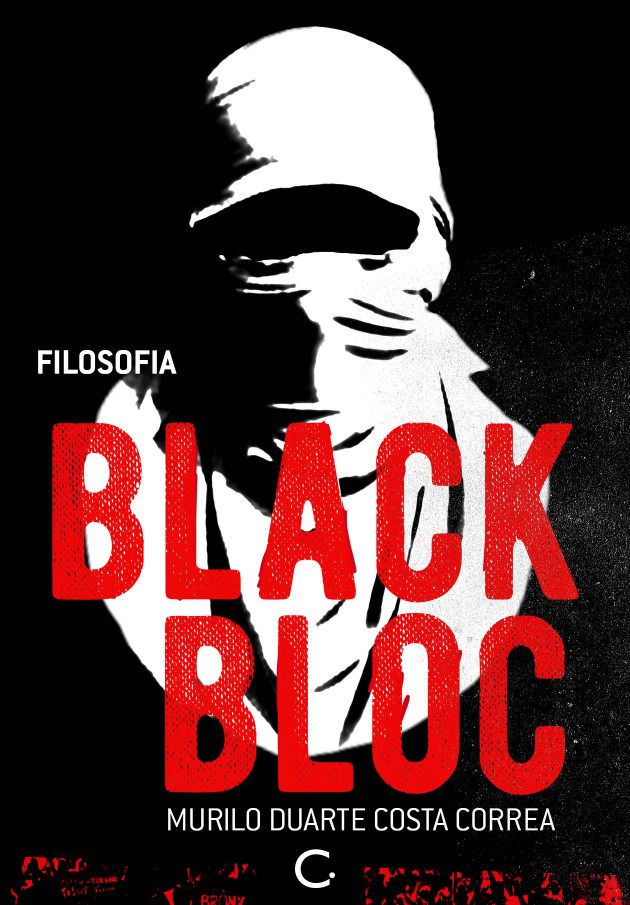
\includegraphics[width=49mm]{./imgs/blackbloc.jpg}
\end{center}

\hspace*{-7cm}\hrulefill\hspace*{-7cm}

\medskip

\noindent{}Em junho de 2013, na maior erupção social recente, o Black bloc ganhou os holofotes como nova prática de luta. Analistas foram forçados a compreendê-lo, normalmente municiando um repertório conceitual que não entendia o Black bloc em seus próprios termos. {\slsc{Filosofia Black bloc}} procura suprir essa carência e conceber um arcabouço teórico que permita abordar o Black bloc como fenômeno. Produzir, no pensamento, uma filosofia Black bloc.

%\hspace{.5cm}
\vfill

\hspace*{-.4cm}\begin{minipage}[c]{1\linewidth}
\small{
{\Formular{\textbf{
\hspace*{-.1cm}Título: Filosofia Black bloc\\
Autor: Murilo Duarte Costa Correa\\ 
Páginas: 166\\
Formato: 12,7x19,1cm\\
Preço: R\$ 46,90\\
ISBN: 978-85-9582-056-2\\
Disponibilidade: Disponível a partir de abril
}}}}
\end{minipage}

\pagebreak

\hspace{.5cm}

\begin{center}
\hspace*{-4cm}\raisebox{5.8cm}{\rotatebox[origin=t]{90}{\Formular{\textbf{Lançamento}}}}
\hspace*{4cm}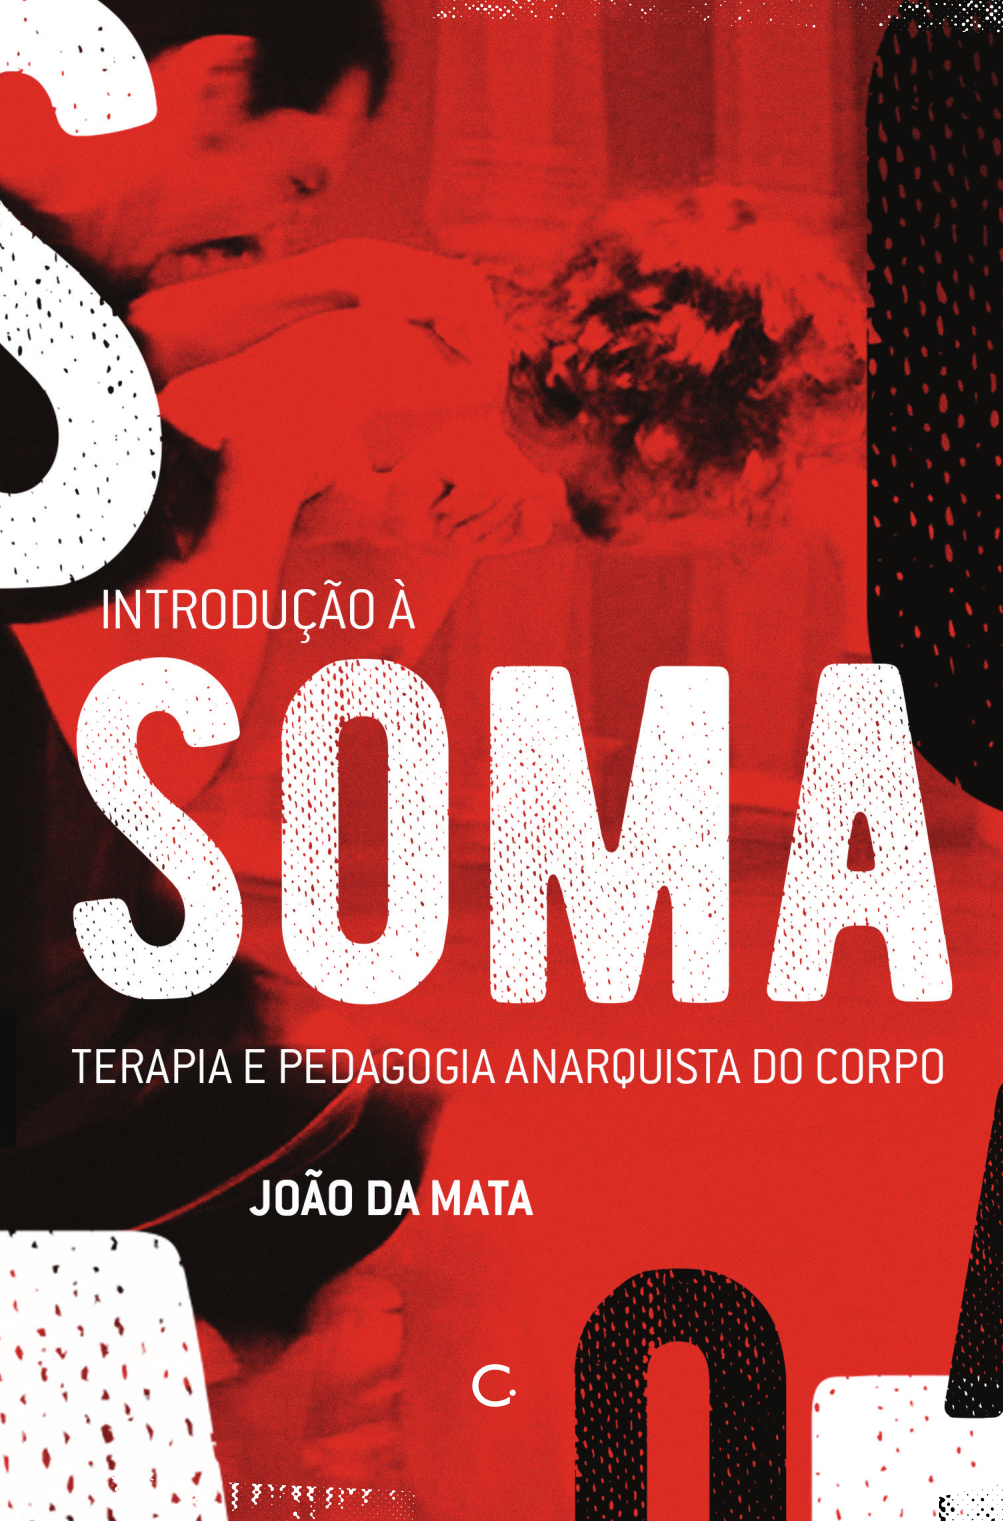
\includegraphics[width=48mm]{./imgs/soma.jpg}
\end{center}

\hspace*{-7cm}\hrulefill\hspace*{-7cm}

\medskip

\noindent{}{\slsc{Introdução à Soma}} trata de um processo terapêutico realizado em grupo, corporal, que busca no pensamento anarquista uma crítica às formas de poder impregnadas no comportamento individual. O grupo funciona como um micro"-laboratório social, daí sua originalidade: a terapia é criação de si, em que a construção das práticas de liberdade é o antídoto para os conflitos gerados pelas hierarquias sociais.

\vfill

\hspace*{-.4cm}\begin{minipage}[c]{1\linewidth}
\small{
{\Formular{\textbf{
\hspace*{-.1cm}Título: Introdução à \scalebox{.8}{SOMA}: terapia e pedagogia anarquista do corpo\\
Autor: João da Mata\\ 
Páginas: 106\\
Formato: 12,7x19,1cm\\
Preço: R\$ 42,90\\
ISBN: 978-85-9582-055-5\\
Disponibilidade: Disponível a partir de abril
}}}}
\end{minipage}

\pagebreak
\pagestyle{circuitocat}

\begin{multicols}{2}
\begin{enumerate}
\item A grande marcha, {\Formular{\textbf{Ewerton Martins Ribeiro }}}
\item A loucura branca, {\Formular{\textbf{Jaime Rocha}}}
\item A outra morte de Alberto Caeiro, {\Formular{\textbf{Afonso Henriques Neto}}}
\item A Dialética do gosto, {\Formular{\textbf{Marco Scheinder}}}
\item Adoecer, {\Formular{\textbf{Hélia Correia}}}
\item Almas selvagens, {\Formular{\textbf{André Gardel}}}
\item Até ano que vem em Jerusalém, {\Formular{\textbf{Maria da Conceição Caleiro}}}
\item Cadernos de artista, {\Formular{\textbf{Moisés Alves}}}
\item Cérebro-Ocidente/Cérebro"-Brasil, {\Formular{\textbf{Roberto Corrêa dos Santos}}}
\item Nove tiros em Chef Lidu, {\Formular{\textbf{Paula Bajer Fernandes}}}
\item Comunidades sem fim
\item Coletivos
\item DJs
\item Dezembro, {\Formular{\textbf{Ana Tereza Salek}}}
\item Os tigres cravaram as garras no horizonte, {\Formular{\textbf{Augusto Guimaraens Cavalcanti}}}
\item No contemporâneo: arte e escritura expandidas, {\Formular{\textbf{Roberto Corrêa dos Santos; Renato Rezende}}}
\item Truques de autor, {\Formular{\textbf{Heleno Bernardi}}}
\item Clínica de artista I, {\Formular{\textbf{Roberto Corrêa dos Santos}}}
\item Clínica de artista II, {\Formular{\textbf{Roberto Corrêa dos Santos}}}
\item Vertigens, {\Formular{\textbf{Fernanda de Mello Gentil}}}
\item Nós somos uma correspondência, {\Formular{\textbf{Fernanda de Mello Gentil}}}
\item Amarração, {\Formular{\textbf{Renato Rezende}}}
\item Conversas com curadores e críticos de arte
\item Experiência e arte contemporânea
\item Romance, {\Formular{\textbf{Caio Meira}}}
\item Auréola, {\Formular{\textbf{Renato Rezende}}}
\item Cosmocrunch, {\Formular{\textbf{Maria Dolores Wanderley}}}
\item Preces para a amiga submersa, {\Formular{\textbf{Lucia Castello Branco}}}
\item Pequena coleção de grandes horrores, {\Formular{\textbf{Luiz Brás}}}
\item Nós, o outro, o distante na arte brasileira contemporânea, {\Formular{\textbf{Marisa Flórido Cesar}}}
\item Lira dos sentidos, {\Formular{\textbf{Carlos Henrique Costa}}}
\item Rasga-mortalha: poemas dos outros, {\Formular{\textbf{W. B. Lemos}}}
\item Os nomes, {\Formular{\textbf{Rogério Luz}}}
\item N’Ágorainda, {\Formular{\textbf{Naila Rachid}}}
\item O ser-se, {\Formular{\textbf{Júnia Azevedo}}}
\item A reflexão atuante, {\Formular{\textbf{Sergio Cohn}}}
\item Intervenções críticas, {\Formular{\textbf{Josefina Ludmer}}}
\item O homem mais portátil do mundo, {\Formular{\textbf{Arturo Carrera}}}
\item O capitão Nemo e eu, {\Formular{\textbf{Alfredo Prior}}}
\item Notas, disparos, sublinhados, {\Formular{\textbf{María Moreno}}}
\item Naxos, {\Formular{\textbf{Elsa Cross}}}
\item Diário em progresso, {\Formular{\textbf{Alex Frechette}}}
\item Em caso de emergência pare o tempo, {\Formular{\textbf{Gab Marcondes}}}
\item 1,68 x 1,81, {\Formular{\textbf{Maria André Leite}}}
\item Do tudo e do todo, {\Formular{\textbf{Cláudio Oliveira}}}
\item S.O.S. Poesia, {\Formular{\textbf{Renato Rezende; Dirk Vollenbroich}}}
\item O olho do lince, {\Formular{\textbf{Guilherme Zarvos}}}
\item Diário para descolorir, {\Formular{\textbf{Alex Frechette}}}
\item A pequena voz do mundo, {\Formular{\textbf{Diana Bellessi}}}
\item Amazônia \& Co., {\Formular{\textbf{Rafael Cippolini}}}
\item Fala, poesia, {\Formular{\textbf{Tamara Kamenszain}}}
\item Suturas. Um breviário, {\Formular{\textbf{Daniel Link}}}
\item Repetir, {\Formular{\textbf{Katia Maciel}}}
\item Coreografia (Orelhas contemporâneas), {\Formular{\textbf{André Parente}}}
\item Amor: verso: reverso (Orelhas contemporâneas), {\Formular{\textbf{Luiz Sérgio de }}}Oliveira
\item Saudades de um punhal (Orelhas contemporâneas), {\Formular{\textbf{Leila Danziger}}}
\item Gravidade (Orelhas contemporâneas), {\Formular{\textbf{Katia Maciel}}}
\item Artexperiência contemporânea (Orelhas contemporâneas), {\Formular{\textbf{Renato }}}Rezende
\item Práticas contemporâneas do mover-se, {\Formular{\textbf{Michelle Sommer}}}
\item Levantem lentamente o lençol, {\Formular{\textbf{Bia Albernaz}}}
\item Escritos sobre fotografia contemporânea brasileira
\item Doctypes, {\Formular{\textbf{Alex Hamburger}}}
\item Quarenta e quatro, {\Formular{\textbf{Mauricio Cardozo}}}
\item Ninfas e Mariposas, {\Formular{\textbf{Leonardo Toledo}}}
\item Lab Criativo / Creative Lab
\item Quase-poesia, {\Formular{\textbf{Jerson Lima Silva}}}
\item Música Chama, {\Formular{\textbf{Pedro Sá Moraes; Eduardo Guerreiro B. Losso}}}
\item Viventes de Saturno, {\Formular{\textbf{Carlos Frederico Manes}}}
\item Esperando a hora da Stella, {\Formular{\textbf{Maria Dolores Wanderley}}}
\item Falar o que seja é inútil – ou sobre desconsiderações, {\Formular{\textbf{Carlos Alberto Gianotti}}}
\item Lótus molotov, {\Formular{\textbf{Leonardo Toledo}}}
\item Outras margens, {\Formular{\textbf{Sergio Cohn}}}
\item Formas híbridas, {\Formular{\textbf{Rafael Gutiérrez}}}
\item Fornicar e matar e outros ensaios, {\Formular{\textbf{Laura Klein}}}
\item Cores cobras pincéis cães, {\Formular{\textbf{Eduardo Stupía}}}
\item Lasca de breu, {\Formular{\textbf{Guilherme Delgado}}}
\item O tropo tropicalista, {\Formular{\textbf{João Camillo Penna}}}
\item Leituras furadas, {\Formular{\textbf{Luis Felipe Fabre}}}
\item Escrever sobre escrever poesia, {\Formular{\textbf{Eduardo Milán}}}
\item A liberação da mosca, {\Formular{\textbf{Luigi Amara}}}
\item Mudança, {\Formular{\textbf{Verónica Gerber Bicecci}}}
\item Onde late um cachorro doido, {\Formular{\textbf{Moisés Alves}}}
\item Daniel Acosta
\item Éter, {\Formular{\textbf{António Cabrita}}}
\item Noturno Europeu, {\Formular{\textbf{Rui Nunes}}}
\item Café irlandês, {\Formular{\textbf{Barbosa Lagos}}}
\item Voo, {\Formular{\textbf{Ana Paula Simonaci}}}
\item Fim do Infante, {\Formular{\textbf{Marina Marcondes Machado}}}
\item 2013, memórias e resistências, {\Formular{\textbf{Camila Jourdan}}}
\item Escrito e dirigido por Moisés Alves, {\Formular{\textbf{Moisés Alves}}}
\item Coisas que fiz e ninguém notou mas que mudaram tudo, {\Formular{\textbf{Moisés Alves}}}
\item A cena lenta, {\Formular{\textbf{Cláudio Oliveira}}}
\item Copa pra quem? Olimpíadas pra quem?, {\Formular{\textbf{Alex Frechette}}}
\item O fantasma de um nome (poesia, imaginário, vida), {\Formular{\textbf{Jorge Monteleone}}}
\item Peso Morto, {\Formular{\textbf{João Felipe Gremski}}}
\item Romance de asilo, {\Formular{\textbf{André Monteiro}}}
\item Quem apaga a luz sou eu, {\Formular{\textbf{Magda Romano}}}
\item As artes do cover, {\Formular{\textbf{Henrique Saidel}}}
\item Frestas, {\Formular{\textbf{André Gardel}}}
\item O antes é o depois, {\Formular{\textbf{Guidi Vieira}}}
\item Humano, {\Formular{\textbf{Pedro Poeta}}}
\end{enumerate}
\end{multicols}

\pagebreak
